\section{Signalübertragung}
Um digitale Signale zu übertragen in einem Differenzsignal, sollten sich die Energie von Mark (1) Space (0) maximal unterscheiden.
\[
s_2(t) = -s_1(t)
\]

\subsubsection{Unipolar NRZ, NRZ-L}\script{93}
Unipolar Non-Return-To-Zero Leitungscode:\\
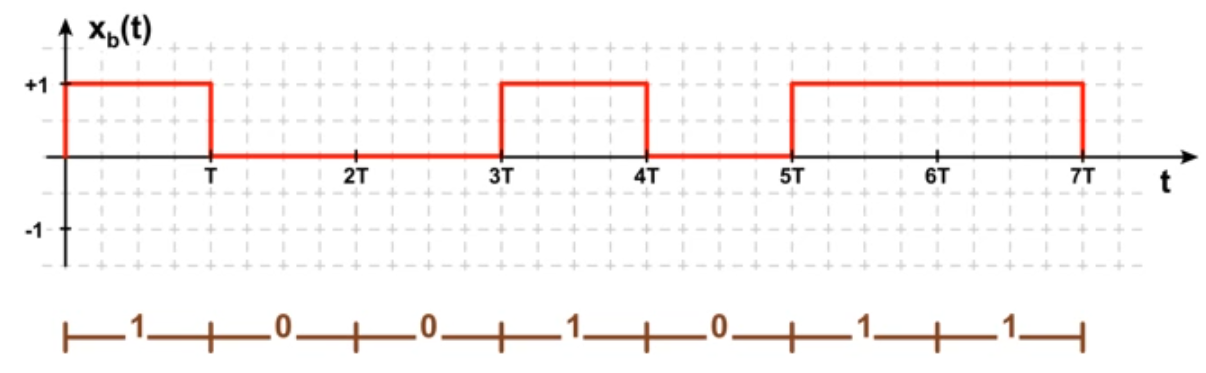
\includegraphics[width=0.6\columnwidth]{Images/nrz}

Verbesserung des NRZ können durch \textbf{Scrambling}, \textbf{Bitstopen} oder \textbf{8b/10b-Codierung} erreicht werden.

\subsubsection{Bipolar NRZ}\script{95}
Bipolar NRZ Leitungscode:\\
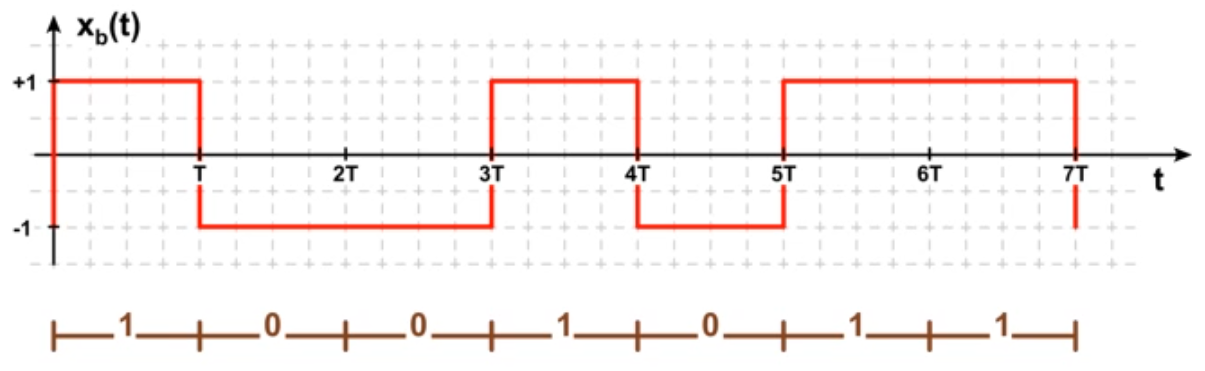
\includegraphics[width=0.6\columnwidth]{Images/nrz1}

\subsubsection{NRZI}\script{96}\\
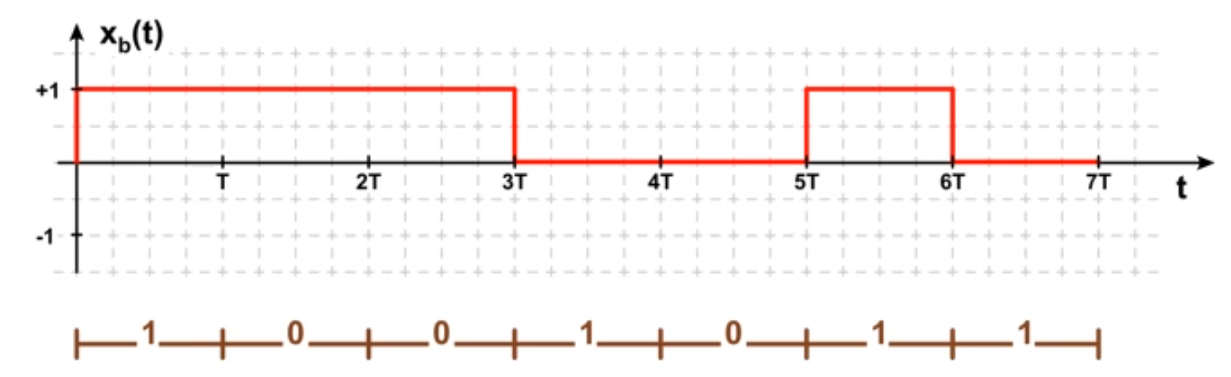
\includegraphics[width=0.6\columnwidth]{Images/nrzi}

\subsubsection{Unipolar RZ}\script{97}\\
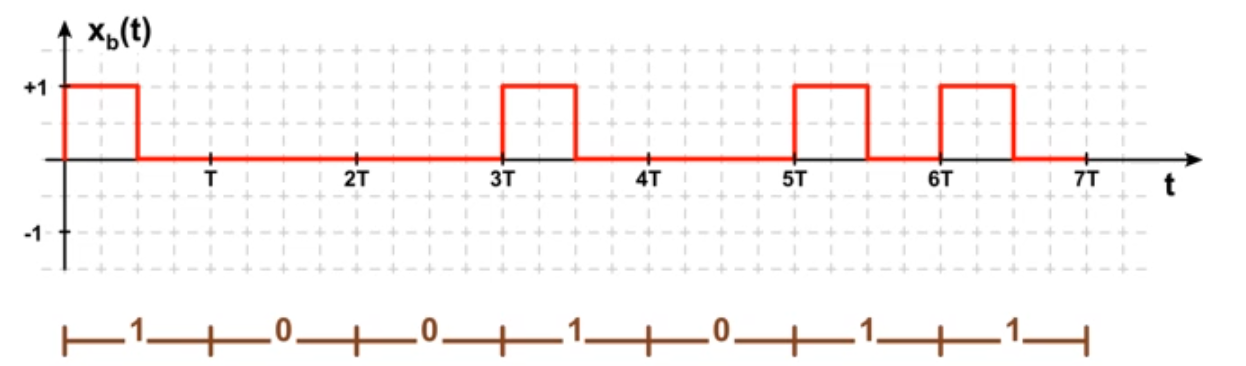
\includegraphics[width=0.6\columnwidth]{Images/urz}

\subsubsection{Bipolar RZ}\script{97}\\
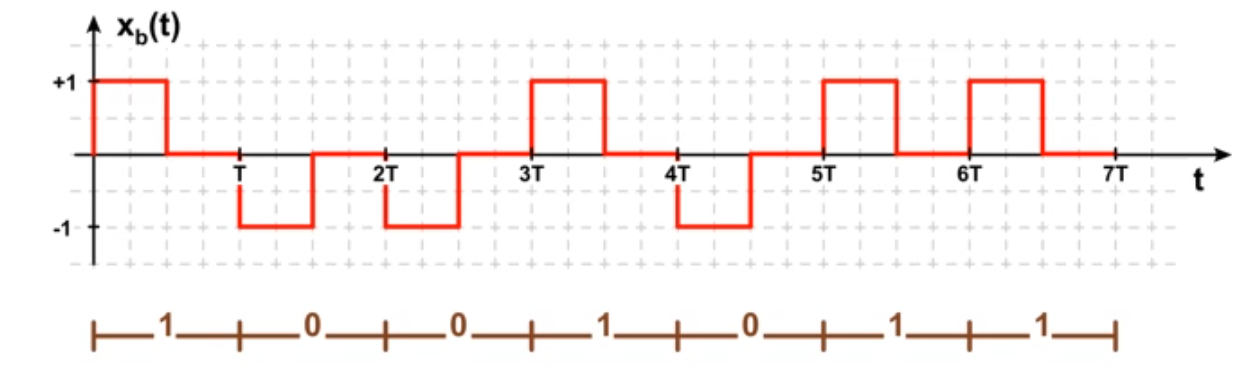
\includegraphics[width=0.6\columnwidth]{Images/brz}

\subsubsection{AMI}\script{98}
Alternative Mark Inversion\\
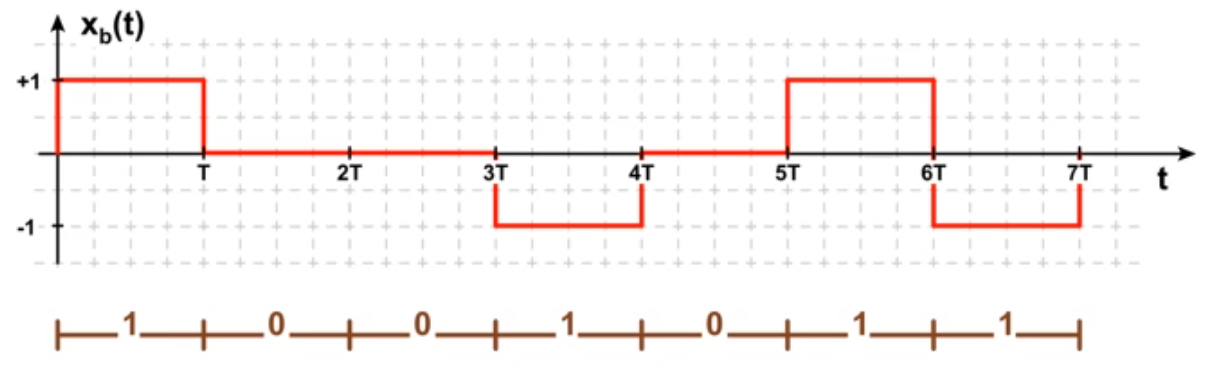
\includegraphics[width=0.6\columnwidth]{Images/ami}

\subsubsection{Manchester Code}\script{99}
Auch Split-Phase, Biphase Level\\
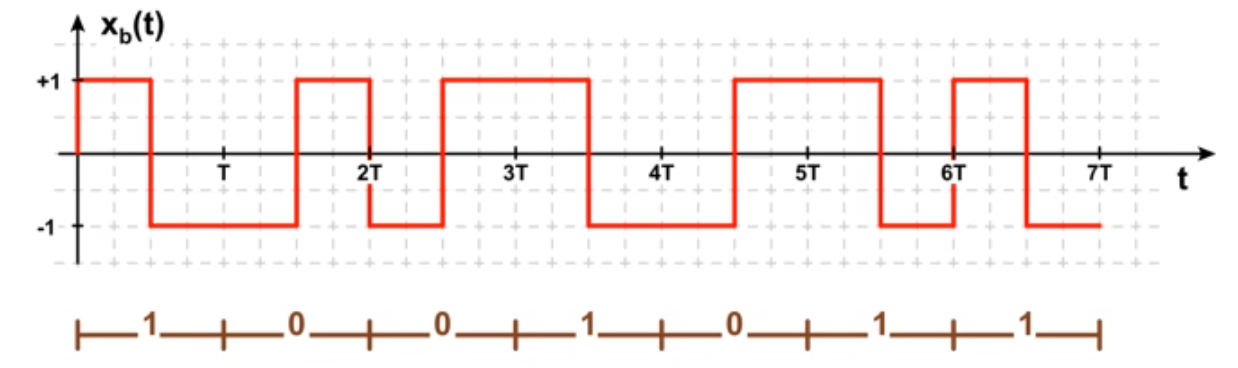
\includegraphics[width=0.6\columnwidth]{Images/manchester}

\subsubsection{MLT3}\script{99}\\
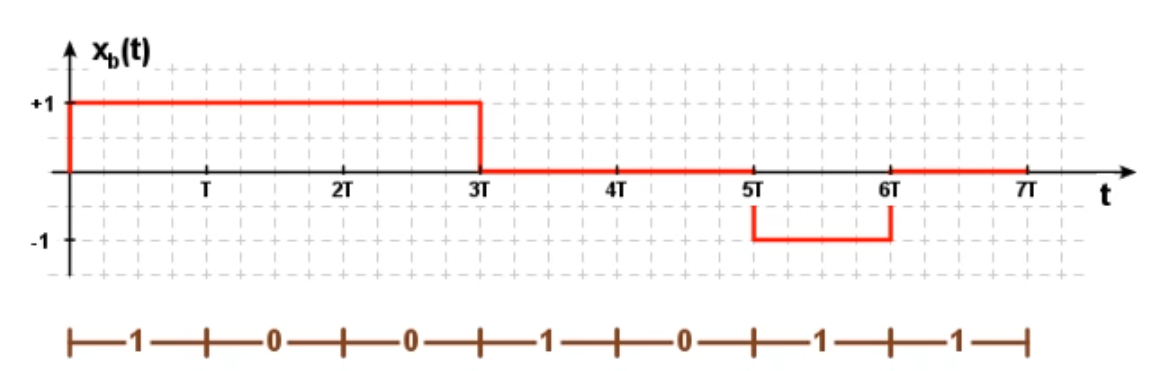
\includegraphics[width=0.6\columnwidth]{Images/mlt3}

\subsubsection{PAM5}\script{101}\\
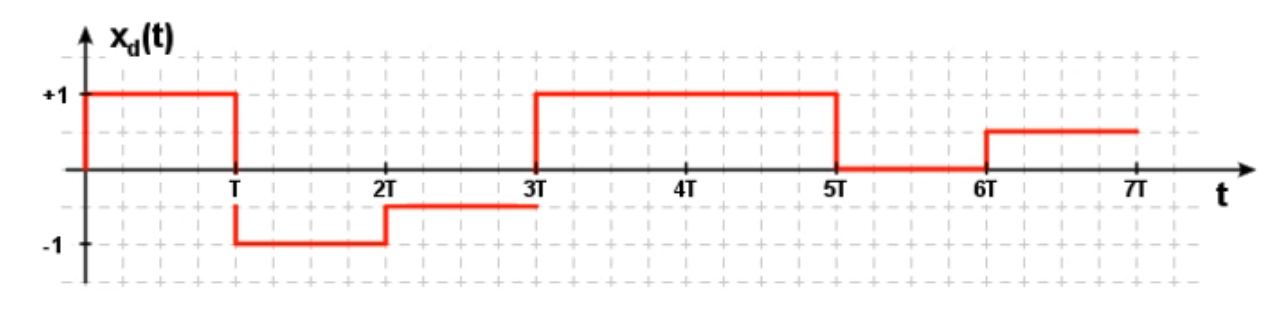
\includegraphics[width=0.6\columnwidth]{Images/pam5}


\subsection{Bandbreitenbedarf}\script{102}
Der minimale Bandbreite $B_d$ [Hz] kann abgeschätzt werden mit $B_d = \frac{f_s}{2}; f_s = \frac{1}{T_s}$

\subsection{Äquivalente Basisbanddarstellung von Bandpasssignalen} 
Bei QAM werden zB für QAM-16 $2^n \rightarrow n = 4Bit/Symbol$ übertragen. Somit werden für Datenrate $d =10kBit/s$ $\frac{d}{n} = 2500Symbole/s$ übertragen \script{114}\\
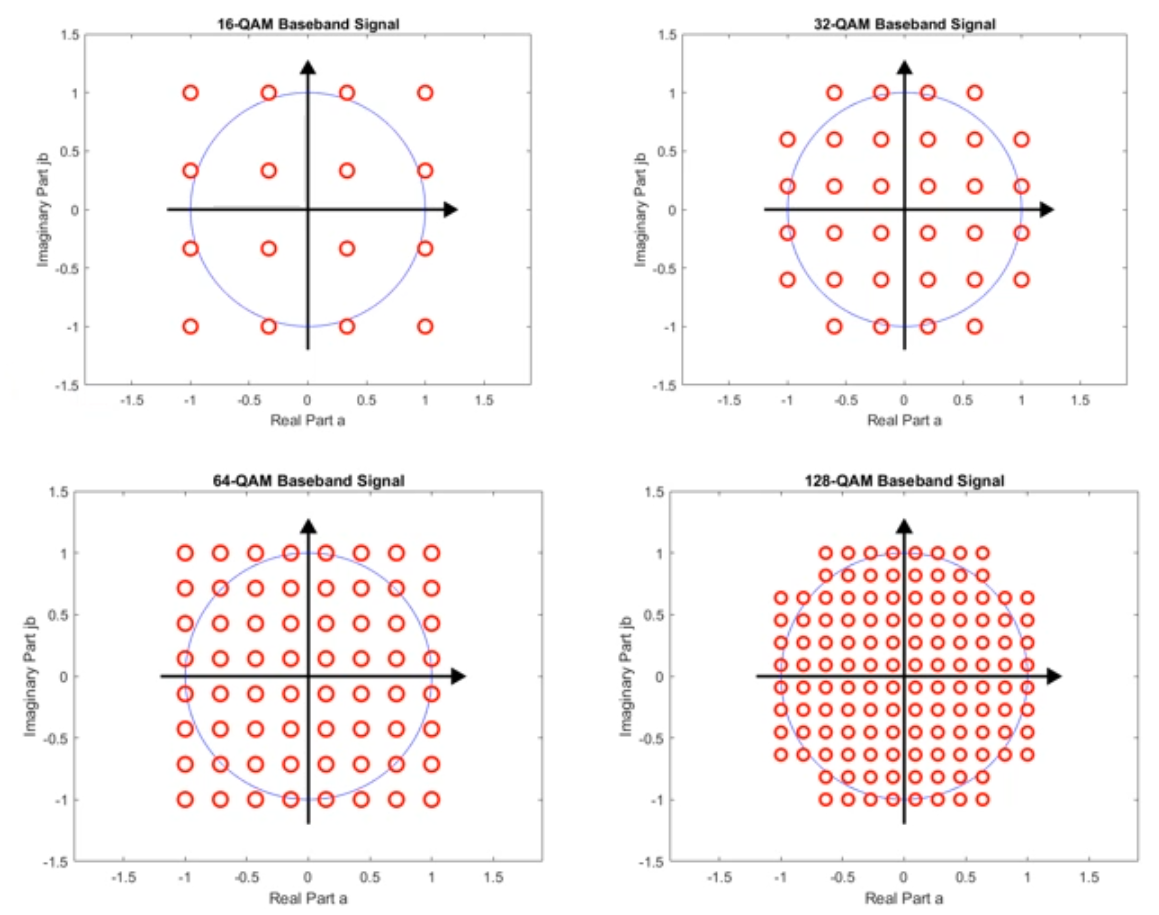
\includegraphics[width=\columnwidth]{Images/qam_basisdarstellung}

\subsection{Pulsformfilter}\script{104}
Um Bandbreite bei der Übertragung einzusparen, werden Rechtecks Signale, wie sie bei der PCM (Pulse-Code-Modulation) vorkommen, schon beim Sender mit einem Filter Abgeflacht, dadurch hat man die physikalische Bandbreite des Kanals unter eigener Kontrolle.

\subsubsection{Raised-Cosine Puls}
Ein beliebter Pulseformfilter ist Raised-Cosine Pulse \script{105} welcher definiert ist durch 
\[
h(t) = \sinc\left(\frac{\pi}{T}t\right)\cdot\frac{\cos(\alpha\frac{\pi}{T}t)}{1- (\frac{2\alpha\pi}{T}t)^2}
\]
Dadurch lassen sich die spektral Bandbreite beschränken und trotzdem beleibt die übertragenen Pulse zum optimalen Zeitpunkt der Auswertung frei von Intersymbol-Interferenz.
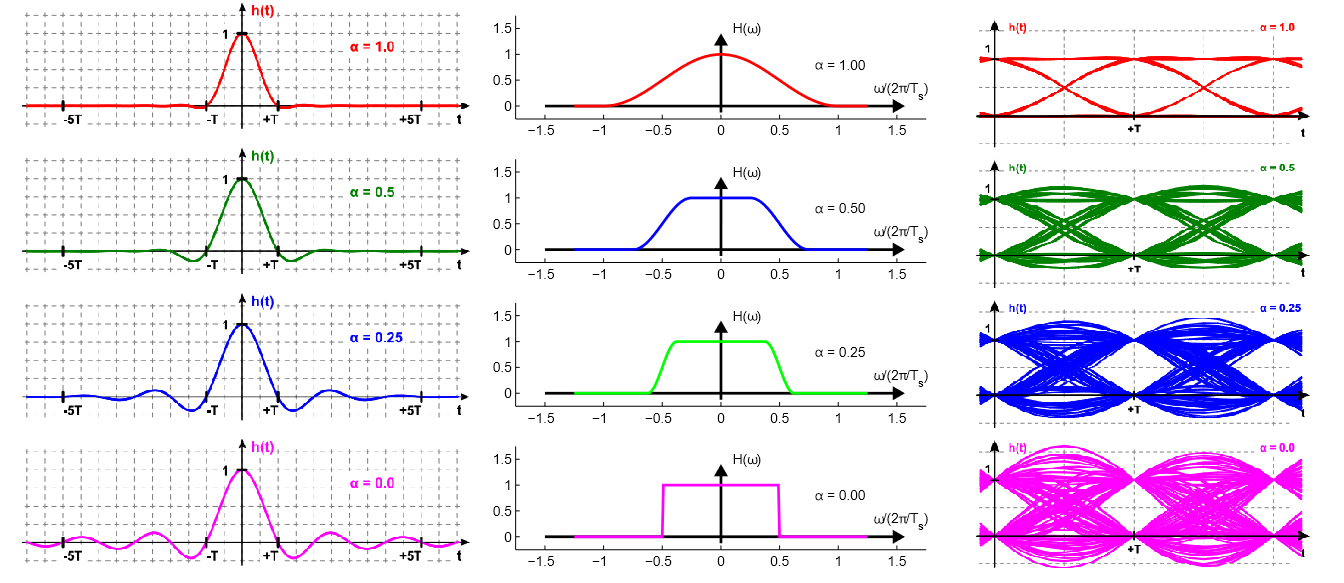
\includegraphics[width=\columnwidth]{Images/raised-cosine_pulse}
Die \textbf{Symbolrate} mit gegebenen Roll-off-Faktors $\alpha$ und einer Bandbreite $B$, dabei ist die Übertragungsrate maximal bei $\alpha=0$ und minimal bei $\alpha=1$ 
\[
d = \frac{2B}{1 + \alpha}
\]
\textbf{Beispiel}
Die Nutzdaten mit $10MHz$ bei 8b/10b-codierten NRZ-Signal sind $d_d = d \cdot \frac{8}{10} = 16MBit/s$, bei Manchester-Code $d_d = d \cdot \frac{1}{2} = 10MBit/s$